\section{纹理坐标的插值}

类似于着色时有“逐顶点着色”和“逐片元着色”之分,纹理映射有同样的问题。由于纹理的颜色变化往往不是连续的,我们通常在三角面上插值顶点的纹理坐标而不是纹理颜色,换言之,对于一个三角面,首先通过纹理坐标映射将三个顶点的世界坐标转换为纹理坐标,随后在光栅化时通过重心插值取得每个像素处的纹理坐标,再查询纹理贴图得到该处应有的颜色。
\begin{Figure}[纹理坐标的循环边界]
    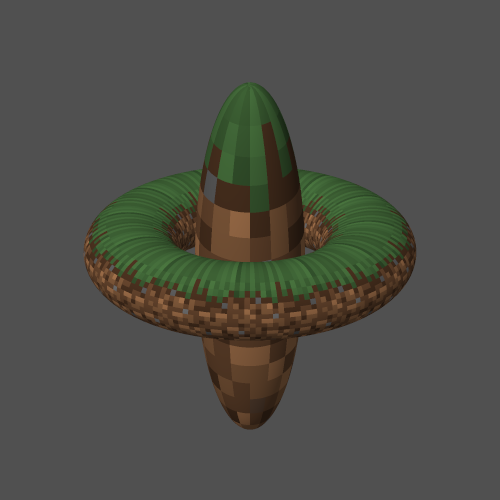
\includegraphics[width=6.5cm]{RasterizationIOW/SphereRingTexture.png}
\end{Figure}

然而,纹理坐标的插值在有些情况下会存在问题。例如在球面投影和柱面投影中,当同一个三角面的两个顶点的经度$\phi\in[-\pi,\pi]$跨越循环边界时,比如$\phi_1=0.97\pi$而$\phi_2=-0.99\pi$,两者的中点应该是$\phi=0.99\pi$吗,但是,插值出的中点却是$\phi=-0.01\pi$,插值会跨越大半个球面而不是走跨越边界的最短路径!为此,我们需要谨慎的保证同一个三角面的顶点经度不可以跨越边界,这个例子中,可以令$\phi_1=0.97\pi$和$\phi_2=1.01\pi$,插值时就不会产生问题了。不过这会导致$u$超出$[0,1]$的范围,这可以通过为纹理坐标$u,v$设置循环边界解决,形象的说,想象纹理空间并不仅仅只有$[0,1]^2$的范围,而是用$[0,1]^2$的图案像瓷砖一样铺满了整个空间。

纹理坐标使用循环边界不仅仅可以用于满足上述经度插值中的技术需要,还可以更好满足实际需要。例如在\cref{fig:纹理坐标的循环边界}中,圆环和椭球都使用了柱坐标投影,然而,圆环的的$u$被放大了$12$倍,这意味着其在经度方向的纹理其实是由$12$张贴图拼接而来,避免了小方格被过度拉伸。

纹理坐标的插值还会在立方体投影中出现问题,试想,当同一个三角面的顶点分别归属于立方体不同面时的贴图时,插值显然会遇到麻烦。简洁的解决方案是:直接对顶点的世界坐标插值,在每个像素处再将世界坐标转换为纹理坐标。当然,我们或许会问,为什么不能对于所有投影方式也这样做?因为至纹理坐标的转换比较耗时,有条件的话避免逐像素的做这个转换。